\subsection{Parser de la regex}
Las expresiones regulares están representadas por una clase a la cual llamamos Regex.
Cada instancia tiene 3 atributos:
\begin{itemize}
	\item nombre = $OR, CONCAT, \ldots , SIMOBOLO$
	\item valor = x en el caso en el que la regex representa un símbolo (con x perteneciente al listado de caracteres válido),`` '' en el resto de los casos.
	\item argumentos = un arreglo con una única regex si la regex es unaria ($PLUS, STAR$), con \emph{n} regex para $CONCAT$ y $OR$, o [ ] en el caso de los símbolos.
\end{itemize}
La función que parsea la regex: ``parsear\_regex'' se llama recursivamente por cada uno de los argumentos, manteniendo el estado del archivo. Incluímos a continuación un pseudocódigo que captura la idea del mismo:

\begin{algorithm}
  \begin{algorithmic}
    \Function{parsear\_regex}{archivo}
      \State $l = archivo.leer_linea()$
      \If {($l$ contiene una operacion. I.E, aparece un string encerrado entre ``\{'' y ``\}'')}
        \State $operacion = capturar\_string()$, capturo el string entre ``\{'' y ``\}''
        \If {($operacion$ lleva argumentos)}
          \State \/** $operacion \in \{OR, CONCAT\}$ \/***
          \State $argumentos = [ \ ]$
          \State $n = capturar\_cantidad\_argumentos()$
          \For {$i=1 to n$}
            \State \/** llamo recursivamente por cada argumento\/**
            \State $argumentos.push(parsear\_regex(archivo))$
          \EndFor
        \Else
          \State \/** llamo recursivamente una única vez \/**
            \State $argumentos.push(parsear\_regex(archivo))$
        \EndIf
        \State \/** Calculados los argumentos, puedo terminar de armar la regex \/**
        \State return $Regex(operacion, [ \ ], argumentos)$
      \Else
        \State \/** Estoy leyendo un símbolo \/**
        \State $s = capturar\_simbolo()$
        \State return $Regex('simbolo', s, [ \ ])$
      \EndIf
    \EndFunction
  \end{algorithmic}
\end{algorithm}


\subsection{Armado del autómata finito:}
Para realizar esta función nosotros partimos de un lenguaje regular parseado, el cual está explicado en la sección \textbf{Parseo de Regex}. A este mismo lo leeremos e iremos armando el autómata finito correspondiente.
La forma de generar nuestro autómata finito es por medio del método de Thompson. Básicamente el algoritmo funciona de forma recursiva y lo detallaremos a continuacion:
\begin{itemize}
\item Se fija si debe realizar \textit{CONCAT}, \textit{PLUS}, \textit{STAR}, \textit{OR}, \textit{OPT} o \textit{SIMBOLO}.
\item Si es \textit{SIMBOLO} crea un automata que tiene dos estados y una transición con el símbolo correspondiente.
\item En caso de no ser \textit{SIMBOLO} va mirando los argumentos y, en cada caso, llama recursivamente a la función para que cree el autómata del mismo. Luego dentro del nivel en el que nos encontramos usamos la funcion \textit{armarConcar}, \textit{armarPlus} o \textit{armarOr} según corresponda, de esta manera, cada una se encargarán de armar el autómata tal como lo describe Thompson. Cabe destacar que no hemos hecho un \textit{armarStar} ni \textit{armarOpt}, esto se debe a que el primero sólo agrega una transición más con respecto a \textit{armarPlus}, y el segundo es un caso idéntico al \textit{armarOr} definiendo uno de los parámetros como un automata con transición lambda.
\item En el caso del \textit{CONCAT} y \textit{OR} que pueden tener $n$ argumentos, hemos optado que el \textit{armarConcat} y el \textit{armarOr} sólo puedan ir armando de a dos autómatas y luego, al obtener el armado de ambos, buscar recurisvamente el autómata del siguiente argumento y repite el paso anterior sucesivamente.
\end{itemize}

La explicación de cómo construir el autómata a partir de las expresiones regulares puede ser encontrada en:

\url{https://en.wikipedia.org/wiki/Thompson's_construction_algorithm}

\subsection{Determinizar Autómata:}
En esta función usamos el algoritmo visto en la clase práctica, calculamos las clausuras para cada estado.\newline
Para poder obtener la primera clausura obtenemos el estado inicial y sobre ese aplicamos una clausura lambda y obtenemos el primer conjunto. Luego sobre este conjunto aplicamos la clausura para cada símbolo del autómata no determinístico, sin contar el símbolo $lambda$.\newline
Continuamos analizando como nos indica el algoritmo analizando cada conjunto conseguido para cada símbolo, siempre y cuando no lo hayamos analizado ya.
Finalizando cuando hayamos analizado todos sin obtener nuevos conjuntos sin analizar.\newline
Dejando la teoría del algoritmo a un lado y basandonos en la implementacion, vamos a usar una cola en donde los nuevos conjuntos que vamos a ir consiguiendo lo vamos a meter en la cola, siempre y cuando no se haya analizado ni esté ya dentro de la cola. Luego sacaremos la cabeza de la cola y procederemos a analizar dicho conjunto como se describe en la teoría del algoritmo mencionada.\newline
Además vamos a tener una tabla en donde cada fila es una clausura y cada columna son las letras del alfabeto, de esta forma a pesar de ir desencolando de la cola no vamos a perder las clausuras ya analizadas, porque las necesitamos luego para armar el autómata determinístco. Armar el autómata es sencillo, leeremos la tabla y resolveremos de la misma forma que lo hicimos en clase, poniendo todas las clausuras como estados, el estado inicial será la primer clausura, los estados finales los que en su clausura tienen un estado final del autómata no determinístico, y las transiciones uniendo la tabla, para el estado de la clausura y un símbolo con la clausura que este en su casilla de la tabla.

\vspace{5 mm}
Emularemos a continuación la corrida del algoritmo:
\vspace{5 mm}

\begin{figure}[!h]
  \begin{center}
        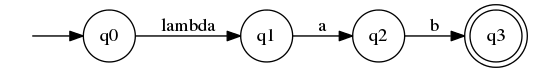
\includegraphics[scale = 0.5]{images/inicial.png}
      \caption{Autómata M}
      \label{fig:contra1}
  \end{center}
\end{figure}

Sea $M = (Q,\Sigma, \delta, q_{0}, F)$ un AFND-$\lambda$, donde:

$Q = [q_{0},q_{1},q_{2},q_{3}]$ ,
$\Sigma = ['a',b']$ ,
$F = [3]$ ,
$q_{0} = 0$ ,
$\delta = [[q_{0},"lambda",q_{1}],[q_{1},'a',q_{2}],[q_{2},'b',q_{3}]]$ .

\vspace{2 mm}
$cola\_conjunto\_clausuras = clausura\_lambda(q_{0}) = [\{q_{0},q_{1}\}]$

\vspace{5mm}

\underline{1ra iteración:}

\vspace{1 mm}

\begin{tabular}{ | l | l | l |}
  \hline
  Conjunto Clausura & a & b \\ \hline
  $\{q_{0},q_{1}\}$ & $\{q_{2}\}$ & $\emptyset$ \\ \hline
\end{tabular}

\begin{itemize}
  \item Popeo el primer estado de $cola\_conjunto\_clausuras$ : $\{q_{0},q_{1}\}$
  \item Completo la fila en la tabla
  \item Agrego los conjuntos calculados a la cola: $[\{q_{2}\}, \emptyset]$
\end{itemize}


\vspace{2mm}

\underline{2da iteración:}

\vspace{1 mm}

\begin{tabular}{ | l | l | l |}
  \hline
  Conjunto Clausura & a & b \\ \hline
  $\{q_{0},q_{1}\}$ & $\{q_{2}\}$ & $\emptyset$ \\ \hline
  $\{q_{2}\}$ & $\emptyset$ & $\{q_{3}\}$ \\ \hline
\end{tabular}

\begin{itemize}
  \item Popeo el primer estado de $cola\_conjunto\_clausuras$ : $\{q_{2}\}$
  \item Completo la fila en la tabla
  \item Agrego los conjuntos calculados a la cola, si no están en ella ni calculé una fila para ellos anteriormente: $[\{\emptyset, \{q_{3}\}]$
\end{itemize}

\underline{3ra iteración:}

\vspace{1 mm}

\begin{tabular}{ | l | l | l |}
  \hline
  Conjunto Clausura & a & b \\ \hline
  $\{q_{0},q_{1}\}$ & $\{q_{2}\}$ & $\emptyset$ \\ \hline
  $\{q_{2}\}$ & $\emptyset$ & $\{q_{3}\}$ \\ \hline
  $\emptyset$ & $\emptyset$ & $\emptyset$ \\ \hline
\end{tabular}

\begin{itemize}
  \item Popeo el primer estado de $cola\_conjunto\_clausuras$ : $\emptyset$
  \item Completo la fila en la tabla
  \item No generé ningún conjunto nuevo. Por lo tanto no agrego elementos a la cola: $[\{q_{3}\}]$
\end{itemize}

\vspace{2 mm}

\underline{4ta y última iteración:}

\vspace{1 mm}

\begin{tabular}{ | l | l | l |}
  \hline
  Conjunto Clausura & a & b \\ \hline
  $\{q_{0},q_{1}\}$ & $\{q_{2}\}$ & $\emptyset$ \\ \hline
  $\{q_{2}\}$ & $\emptyset$ & $\{q_{3}\}$ \\ \hline
  $\emptyset$ & $\emptyset$ & $\emptyset$ \\ \hline
  $\{q_{3}\}$ & $\emptyset$ & $\emptyset$ \\ \hline
\end{tabular}

\begin{itemize}
  \item Popeo el primer estado de $cola\_conjunto\_clausuras$ : $\{q_{3}\}$
  \item Completo la fila en la tabla
  \item No generé ningún conjunto nuevo. Por lo tanto: $cola\_conjunto\_clausuras = [ \ ]$
\end{itemize}

\vspace{2 mm}

Luego de renombrar los estados, el autómata final obtenido es el siguiente:

\vspace{2 mm}

\begin{figure}[!h]
  \begin{center}
        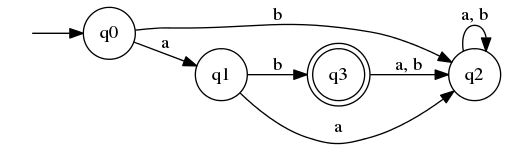
\includegraphics[scale = 0.5]{images/final.png}
      \caption{Autómata M}
      \label{fig:contra1}
  \end{center}
\end{figure}


\subsection{Minimizar Autómata:}
Para minimizar un autómata vamos a usar el algoritmo de minimizar basado en conjuntos. Para esto vamos a empezar partiendo los conjuntos de estados en clases: inicialmente se separaran en estados finales y no finales.\newline
Luego, el algoritmo nos indicaba que deberíamos armar una tabla para cada clase, en donde cada fila es un estado perteneciente a la clase y hay una columna por cada símbolo del alfabeto del autómata inicial. En cada casillero vamos a indicar la clase a la que pertenece el estado destino de la transicion del estado fila y el símbolo columna.\newline
Finalizadas todas las tablas de cada clase, miraremos si dentro de la tabla agarrando cada estado si las filas son iguales o distintas. Si son distintas habrá una nueva clase donde uno de los estados estará en esta nueva clase, y el otro en una distinta, donde agruparemos los que tengan las mismas filas que el primer estado en la primer clase nueva, y los que tengan las mismas fila que el segundo estado en la segunda clase nueva, y así sucesivamente.\newline
La implementación en este caso es bastante trivial a la explicación dada, en donde vamos a armar dichas tablas para cada clase de la partición. Esto lo haremos iterativamente hasta que la nueva partición generada sea igual a la anterior.
Finalmente, para armar el autómata leeremos las tablas de la última partición generada, crearemos los estados correspondientes
y definimos las transiciones con la información almacenada en las tablas.

\subsubsection{Pseudocódigo}

\begin{algorithm}
  \begin{algorithmic}
    \Function{minimizar}{$M = (Q,\Sigma,\delta,q_{0},F)$}
      \State $\Pi = (F, Q \setminus F)$
      \State $\Pi_{new} = new\_partition(\Pi)$
      \While{$\Pi_{new} \neq \Pi$}
        \State $\Pi = \Pi_{new}$
        \State $\Pi_{new} = new\_partition(\Pi)$
      \EndWhile
      \State return $\Pi$
    \EndFunction
  \end{algorithmic}
\end{algorithm}

El resto del algoritmo puede verse en:

\url{http://www.cs.odu.edu/~toida/nerzic/390teched/regular/fa/min-fa.html}


\subsection{Cadena pertenece al lenguaje:}
Lo implementamos lo más directo posible. Esto es, nos paramos en el estado incial y en el primer caracter de la cadena, buscamos la transición en nuestro autómata para ese estado y ese caracter y, una vez encontrado, pasamos al siguiente estado. Repetiremos este paso hasta completar la longitud de la cadena. Una vez finalizada la misma, miramos si el estado en el que estamos parado es un estado final, en caso de serlo la cadena pertence al lenguaje y caso contrario no.\newline
Hay que hacer dos salvedades para esto. La primera es, ¿Qué pasa si la cadena es vacía? Bueno como solución a esto tendremos que chequear la cadena previamente y, en caso de ser vacía, si nuestro estado inicial es también final entonces la cadena será válida, la cadena no pertenecerá al lenguaje en caso contrario. Lo segundo es, ¿Qué pasa si dado un estado y un caracter no encontramos una transición que satisfaga en nuestro conjunto de transiciones? Bueno, esto sólo va a pasar cuando el autómata que estamos recorriendo no es completo, y para solucionarlo bastará con recorrer todas las transiciones y que no se satisfaga la condición, en cuyo caso retornaremos que la cadena no pertenece al lenguaje.

\subsection{Interseccion de dos Autómatas:}
Dados $M_{1} = (Q_{1}, \Sigma_{1}, \delta_{1}, q_{01}, F_{1})$ y $M_{2} = (Q_{2}, \Sigma_{2}, \delta_{2}, q_{02}, F_{2})$,
el algoritmo devuelve un autómata $M = (Q, \Sigma, \delta, q_{0}, F)$ que reconoce el lenguaje $L = L(M_{1}) \cap L(M_{1})$.

En primer lugar calculamos $\Sigma = \Sigma_{1} \cap \Sigma_{2}$

Luego calculamos $Q = \{[q_{1},q_{2}]\}$, donde $q_{1} \in Q_{1} \wedge q_{2} \in Q_{2}$.
(Notemos que $Q$ es un conjunto de pares ordenados de estados)

Calculamos $\delta$ de la siguiente manera:
$([e_{1},e_{2}],a,[e_{3},e_{4}]) \in \delta \iff [e_{1},a,e_{3}] \in \delta_{1} \wedge [e_{2},a,e_{4}] \in \delta_{2}, a \in \Sigma$

$q_{0} = [q_{01},q_{02}]$

$F = [f_{1},f_{2}]$, donde $f_{1} \in F_{1} \wedge f_{2} \in F_{2}$.

Para finalizar y que quede como un autómata comun y no tenga estados con nombre en forma de tuplas, pasamos a renombrar los estados.

Cabe mencionar que este algoritmo genera muchos estados sobrantes. I.E, estados que no son alcanzados desde el estado inicial. Para solucionar esto pasamos a determinizar el nuevo autómata, con lo cual borramos dichos estados y obtenemos el verdadero autómata intersección. Finalmente lo minimizamos.

\subsection{Complemento de un autómata:}
Para esta función necesitamos que todos los estados sean completos. I.E, que para cualquier estado $q \in Q$, y para todo símbolo $s \in \Sigma$ exista exactamente una transición de la forma $(q,s,q_{2})$, con $q_{2} \in Q$. Por lo tanto agregamos un estado \textit{"trampa"} $t$, y nuestro algoritmo se encargará de generar las transiciones ausentes de nuestro autómata y llevarlas a este nuevo estado. Como sabemos este estado \textit{"trampa"} debe cumplir con su definición: no debe ser un estado final y tampoco debe poderse salir de él por medio de alguna transición. Llamaremos $\delta_{t}$ a dichas transiciones agregadas.

Dado un autómata $M = (Q,\Sigma,\delta,q_{0},F)$, el algoritmo calcula en un primer paso un autómata $M_{2} = (Q \cup \{t\}, \Sigma, \delta \cup \delta_{t}, q_{0}, (Q \cup \{t\}) - F) $. Notemos que los nuevos estados finales en $M_{2}$ son todos aquellos estados de $Q$ que no eran finales en $M$, junto con $t$.

Finalmente determinizamos $M_{2}$ para eliminar estados inalcanzables o sobrantes y luego minimizamos el autómata obtenido.

\subsection{Equivalencia de autómatas}
Para poder obtener la equivalencia pensamos diferentes estrategias:
\begin{itemize}
\item La primera fue la de ir recorriendo todos los caminos de los autómatas y ver si pasaban por las transiciones en las cuales ambos tenían el mismo caracter. La descartamos porque era engorrosa y difícil de implementar.
\item La segunda idea que surgió fue la usar el complemento de alguno de los dos autómatas e intersecarlo con el otro, de esta manera, si ambos eran equivalente, el resultado será vacío. Con esto parecía que teníamos resuelto el ejercicio, pero notamos casos bordes donde no se satisfacía muy bien este método. Por ejemplo: ¿Qué pasa si uno de los dos autómatas (A1) era inicialmente vacío y el otro no (A2), y además, tomamos el complemento del último mencionado (A2)? Bueno, al intersecar ambos automatas el resultado sería vacío por definición misma de los conjuntos, y concluiríamos que son equivalentes, lo cual es un error.
\item La tercera y última opción fue la siguiente, llamemos a uno de los dos autómatas A1 y al otro A2. Si ``tomamos el complemento de A2 y lo intersecamos con A1'' (A3), y ``tomamos el complemento de A1 y lo intersecamos con A2'' (A4), entonces si tanto A3 y A4 dieron vacío podremos afirmar que son equivalentes. Se puede ver fácilmente que este caso cubre al mencionado en la \emph{segundo idea}, puesto que si miramos la parte agregada recientemente nos comprobará que no son equivalente. Esto es, tomamos al que inicialmente era vacío (A1) su complemento, esto nos da un automata que acepta todas las cadenas, y lo intersecamos con uno no vacío (A2), el resultado es exactamente el autómata A2. Entonces, dado esta nueva propuesta, podemos concluir que no son equivalente, lo cual efectivamente es verdad. Además, para esta tercera opción, pudimos encontrar una demostración que indica que nuestra propuesta marca formalmente una equivalencia entre ambos autómatas.
Es necesario calcular la unión de ambos alfabetos para que ambos utilicen el mismo.
\end{itemize}
